\hypertarget{rcuflashprog_8h}{
\section{rcuflashprog.h File Reference}
\label{rcuflashprog_8h}\index{rcuflashprog.h@{rcuflashprog.h}}
}
Tool for programming the RCU Flash memory. 



This graph shows which files directly or indirectly include this file:\begin{figure}[H]
\begin{center}
\leavevmode
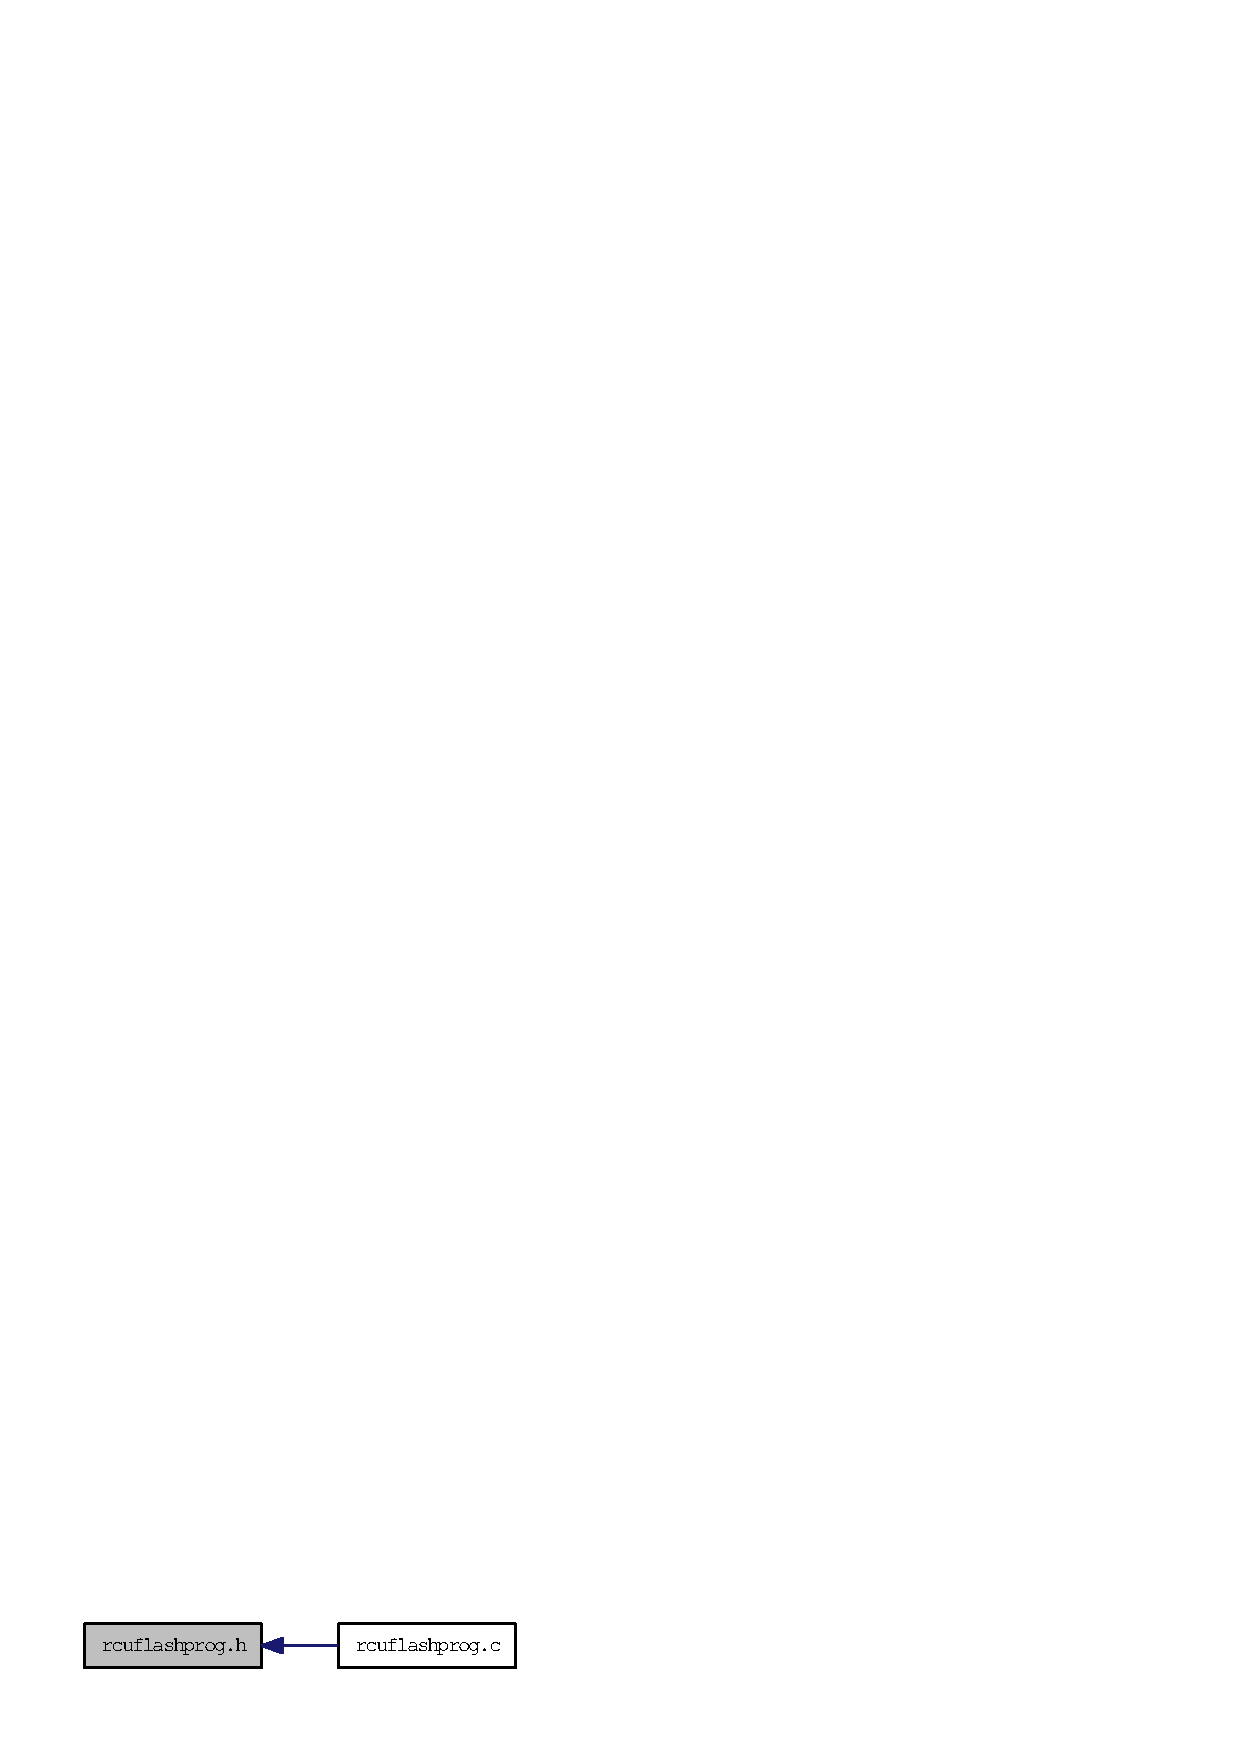
\includegraphics[width=126pt]{rcuflashprog_8h__dep__incl}
\end{center}
\end{figure}
\subsection*{Functions}
\begin{CompactItemize}
\item 
int \hyperlink{rcuflashprog_8h_017730762068a4d5359376e97dac8257}{do\-Init} (char $\ast$conffilename, int \hyperlink{rcuflashprog_8c_a1aabbeb0deebd40a25e329692500bbe}{BB\_\-FLASH})
\item 
int \hyperlink{rcuflashprog_8h_cd9a55766b840c98d87b0ce1a76af867}{do\-Scrubbing} (char $\ast$conffilename, int \hyperlink{rcuflashprog_8c_a1aabbeb0deebd40a25e329692500bbe}{BB\_\-FLASH})
\begin{CompactList}\small\item\em Everything needed for a complete scrubbing is done here. \item\end{CompactList}\item 
int \hyperlink{rcuflashprog_8h_237fcbe3877916a856ff7acf973ee2ba}{do\-Flash\-Frame} (char $\ast$conffilename, int \hyperlink{rcuflashprog_8c_a1aabbeb0deebd40a25e329692500bbe}{BB\_\-FLASH})
\begin{CompactList}\small\item\em The programming of the readframes and writeframes is done here. \item\end{CompactList}\item 
void \hyperlink{rcuflashprog_8h_ed123ebcbaa3f156d6abcbcc17e4c7bc}{build\-Frame\-Filename} (int $\ast$p\-Frameaddr, char $\ast$pnewfilename)
\begin{CompactList}\small\item\em The frameaddress is given with the block, major and minor in an int array as the first parameter. \item\end{CompactList}\end{CompactItemize}


\subsection{Detailed Description}
Tool for programming the RCU Flash memory. 

\begin{Desc}
\item[Author:]Dominik Fehlker \end{Desc}
\begin{Desc}
\item[Date:]\end{Desc}


Definition in file \hyperlink{rcuflashprog_8h-source}{rcuflashprog.h}.

\subsection{Function Documentation}
\hypertarget{rcuflashprog_8h_ed123ebcbaa3f156d6abcbcc17e4c7bc}{
\index{rcuflashprog.h@{rcuflashprog.h}!buildFrameFilename@{buildFrameFilename}}
\index{buildFrameFilename@{buildFrameFilename}!rcuflashprog.h@{rcuflashprog.h}}
\subsubsection[buildFrameFilename]{\setlength{\rightskip}{0pt plus 5cm}void build\-Frame\-Filename (int $\ast$ {\em p\-Frameaddr}, char $\ast$ {\em pnewfilename})}}
\label{rcuflashprog_8h_ed123ebcbaa3f156d6abcbcc17e4c7bc}


The frameaddress is given with the block, major and minor in an int array as the first parameter. 

the second parameter is the filename which contains an \char`\"{}\$\char`\"{} somewhere which is substituted with the frameaddress in this way: \char`\"{}$<$block$>$.$<$major$>$.$<$minor$>$\char`\"{} 

Definition at line 618 of file rcuflashprog.c.

Referenced by do\-Flash\-Frame().\hypertarget{rcuflashprog_8h_237fcbe3877916a856ff7acf973ee2ba}{
\index{rcuflashprog.h@{rcuflashprog.h}!doFlashFrame@{doFlashFrame}}
\index{doFlashFrame@{doFlashFrame}!rcuflashprog.h@{rcuflashprog.h}}
\subsubsection[doFlashFrame]{\setlength{\rightskip}{0pt plus 5cm}int do\-Flash\-Frame (char $\ast$ {\em conffilename}, int {\em BB\_\-FLASH})}}
\label{rcuflashprog_8h_237fcbe3877916a856ff7acf973ee2ba}


The programming of the readframes and writeframes is done here. 

Therefore the framesfile given in the configuration file is read out, and all the given frames there are written to the flash.

\begin{Desc}
\item[Returns:]not used \end{Desc}


Definition at line 163 of file rcuflashprog.c.

References build\-Frame\-Filename(), EXIT\_\-FAILURE, get\-File\-Size(), get\-Frame\-Address\-From\-Line(), get\-Linesnumber\-From\-File(), get\-Lower\-Address(), get\-Upper\-Address(), rcu\-Flash\-Write(), and TRUE.

Referenced by main().

Here is the call graph for this function:\begin{figure}[H]
\begin{center}
\leavevmode
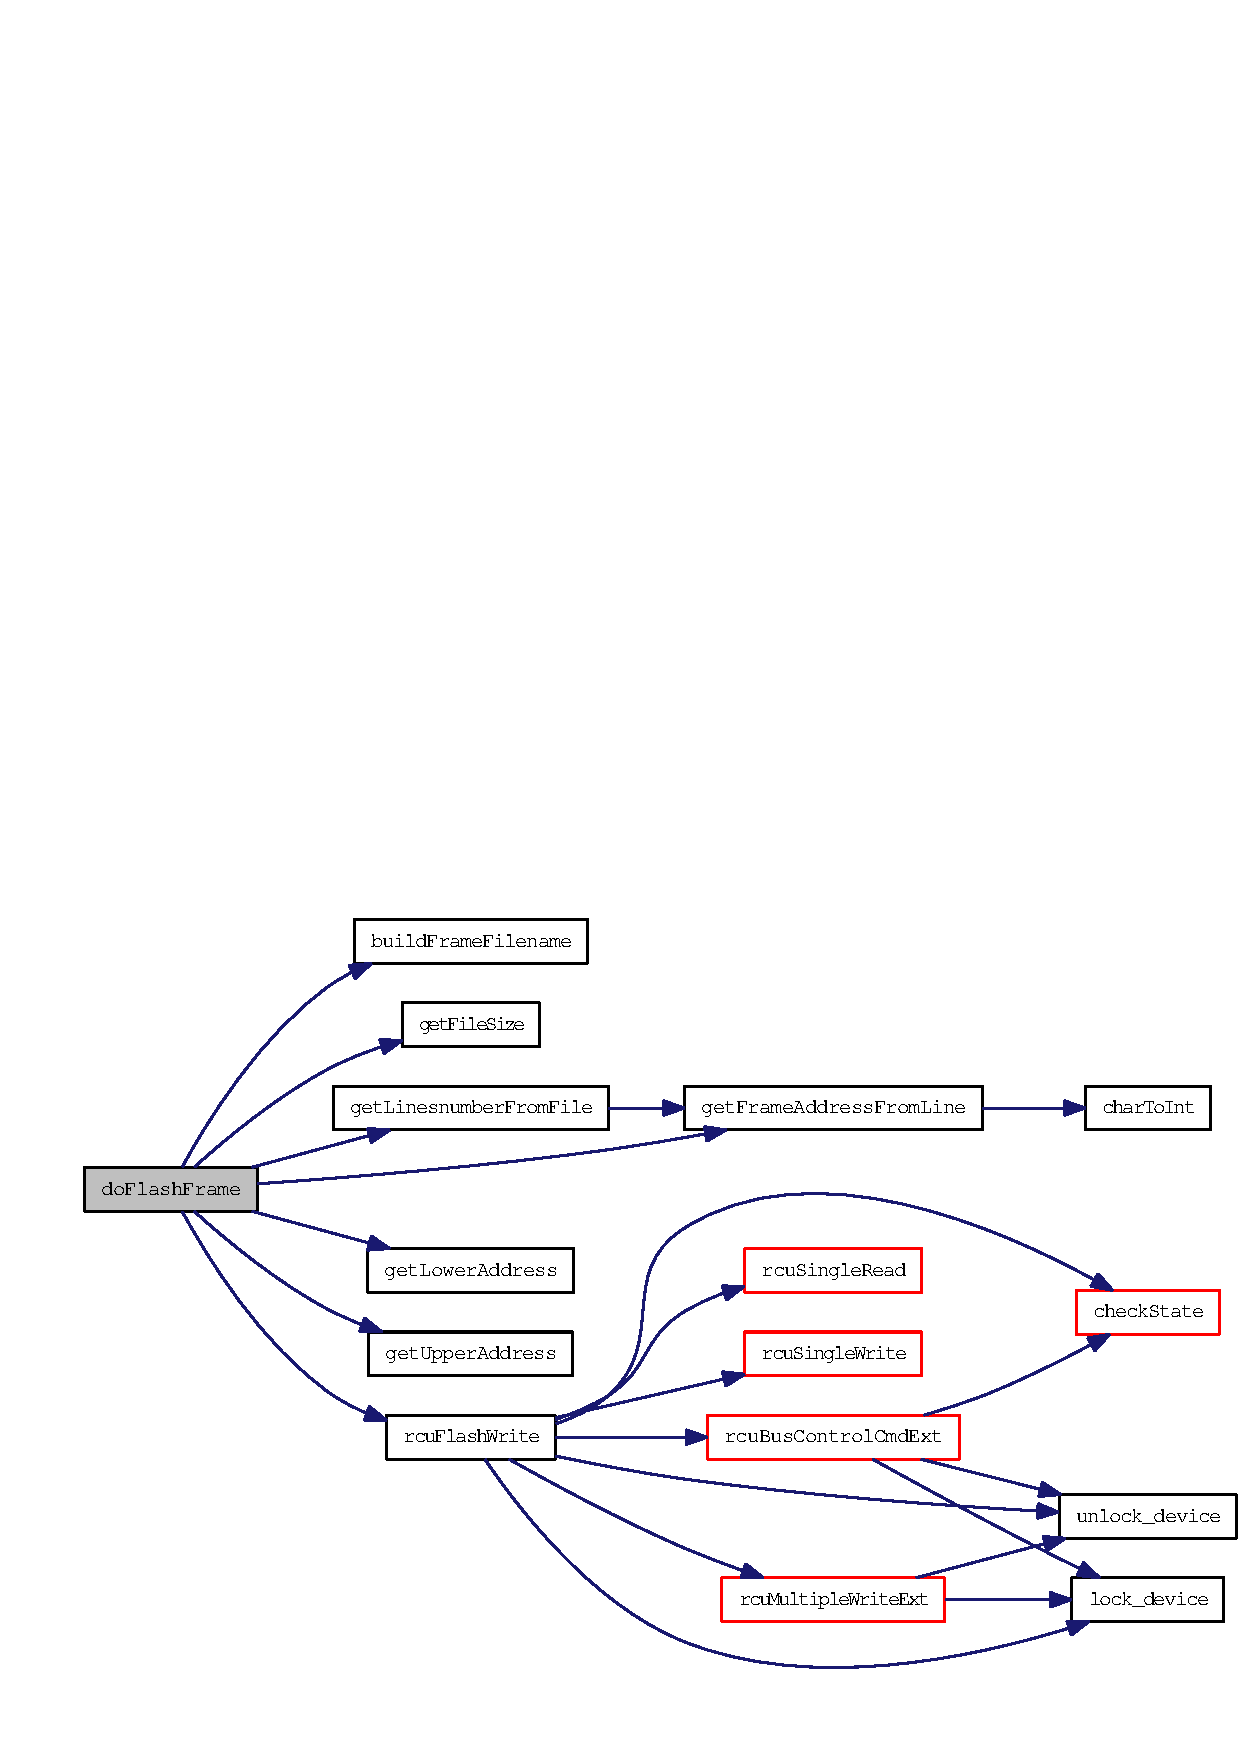
\includegraphics[width=299pt]{rcuflashprog_8h_237fcbe3877916a856ff7acf973ee2ba_cgraph}
\end{center}
\end{figure}
\hypertarget{rcuflashprog_8h_017730762068a4d5359376e97dac8257}{
\index{rcuflashprog.h@{rcuflashprog.h}!doInit@{doInit}}
\index{doInit@{doInit}!rcuflashprog.h@{rcuflashprog.h}}
\subsubsection[doInit]{\setlength{\rightskip}{0pt plus 5cm}int do\-Init (char $\ast$ {\em conffilename}, int {\em BB\_\-FLASH})}}
\label{rcuflashprog_8h_017730762068a4d5359376e97dac8257}




Definition at line 842 of file rcuflashprog.c.

References calculate\-Stop\-Address(), EXIT\_\-FAILURE, get\-File\-Size(), get\-Lower\-Address(), get\-Upper\-Address(), rcu\-Flash\-Write(), and TRUE.

Referenced by main().

Here is the call graph for this function:\begin{figure}[H]
\begin{center}
\leavevmode
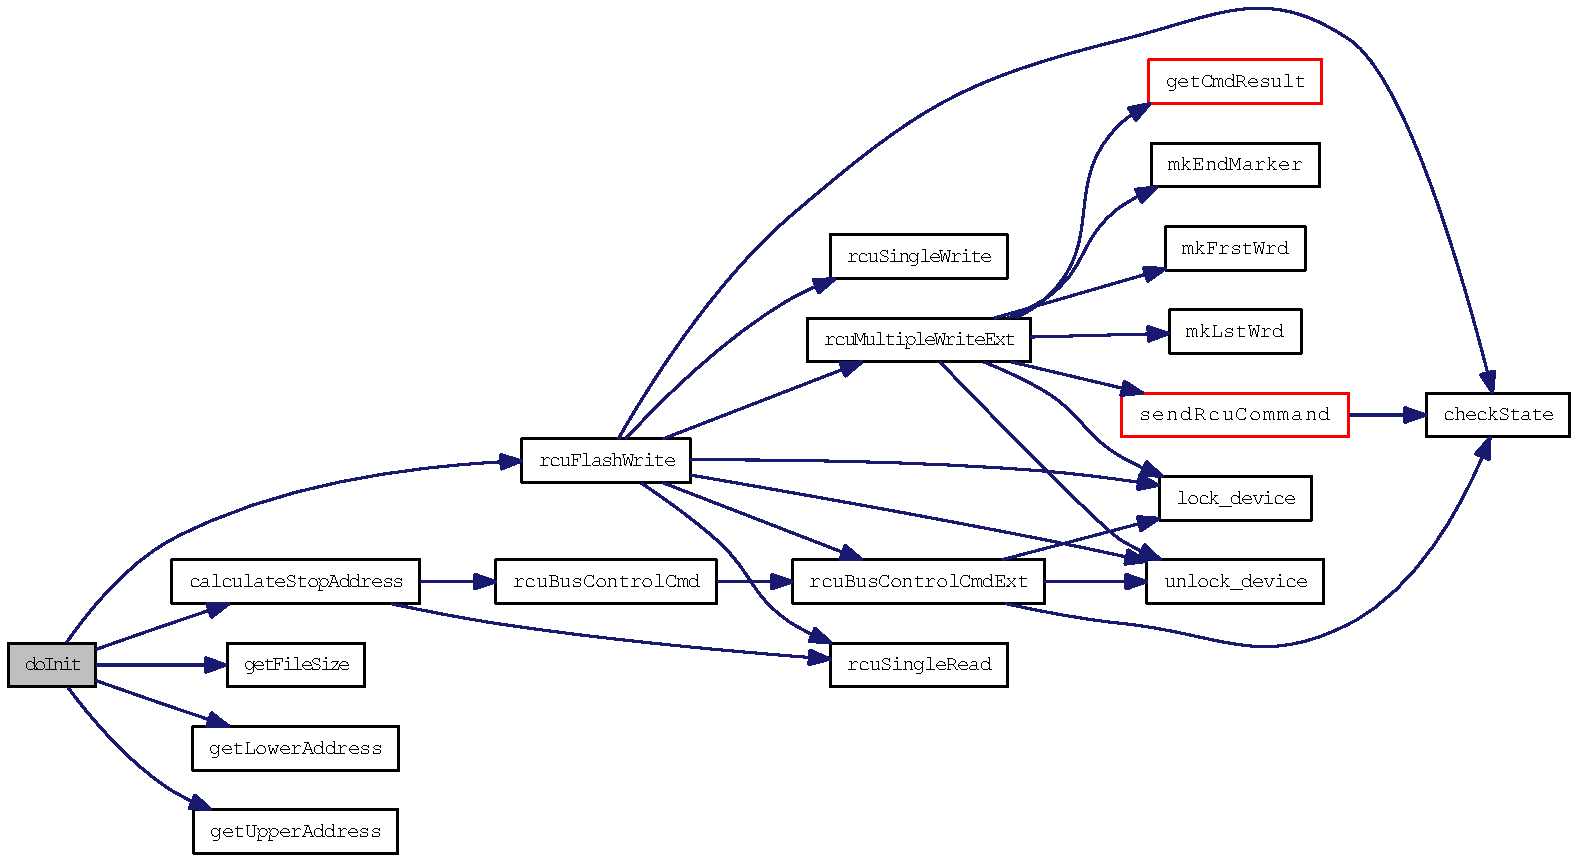
\includegraphics[width=397pt]{rcuflashprog_8h_017730762068a4d5359376e97dac8257_cgraph}
\end{center}
\end{figure}
\hypertarget{rcuflashprog_8h_cd9a55766b840c98d87b0ce1a76af867}{
\index{rcuflashprog.h@{rcuflashprog.h}!doScrubbing@{doScrubbing}}
\index{doScrubbing@{doScrubbing}!rcuflashprog.h@{rcuflashprog.h}}
\subsubsection[doScrubbing]{\setlength{\rightskip}{0pt plus 5cm}int do\-Scrubbing (char $\ast$ {\em conffilename}, int {\em BB\_\-FLASH})}}
\label{rcuflashprog_8h_cd9a55766b840c98d87b0ce1a76af867}


Everything needed for a complete scrubbing is done here. 

All necessary Information is read out from the given configfile.

\begin{Desc}
\item[Returns:]not used \end{Desc}


Definition at line 649 of file rcuflashprog.c.

References calculate\-Stop\-Address(), EXIT\_\-FAILURE, get\-File\-Size(), get\-Lower\-Address(), get\-Upper\-Address(), rcu\-Flash\-Write(), and TRUE.

Referenced by main().

Here is the call graph for this function:\begin{figure}[H]
\begin{center}
\leavevmode
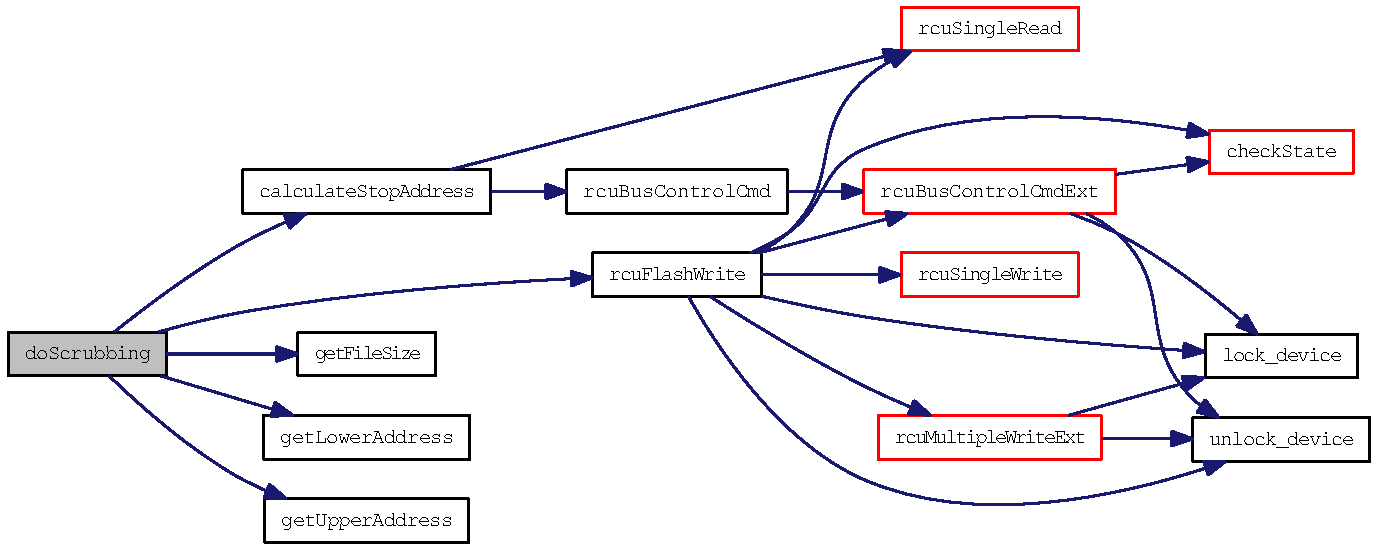
\includegraphics[width=349pt]{rcuflashprog_8h_cd9a55766b840c98d87b0ce1a76af867_cgraph}
\end{center}
\end{figure}
